% --*- coding:utf-8-unix mode:latex -*--
%\include{begin}
%%%%%%%%%%%%%%%%%%%%%%%%%%%%%%%%%%%%%%%%%%%%%%%%%%%%%%%%%%%%%%%%%%%%%%%%%%%%%%%

\section{退所式}

\subsection{日時・場所}
\begin{tabular}{p{2zw}rp{38zw}}
  日時 & : & 2019年4月6日(土) 11:25 $\sim$ 11:55\\
  場所 & : & 体育館
\end{tabular}

\subsection{タイムスケジュール}
% 時刻は必ず4桁(00:00)で書くこと!!!
\begin{longtable}{p{3zw}p{39zw}}
  11:25 & \textbf{◎ トイレ休憩(15分間)} \\
        & \ \ \textbullet \ \ 司会(新川,貞松)はトイレ休憩のアナウンスを行う\\
        & \ \ \textbullet \ \ 司会者は整列をするように促す\\
        & \ \ \textbullet \ \ 日下はこのとき幡多職員さんを呼びに行く \\
        & \ \ \textbullet \ \ 各班のスタッフはプラカードを持ち一列に整列させ,全員が揃った班はその場に座る \\\\

  11:40 & \textbf{◎ Flying Fish斉唱} \\
  	    & \ \ \textbullet \ \ 小島はFlying Fishを流す \\\\

  11:46 & \textbf{◎ 代表挨拶(宮尾)} \\
	    & \ \ \textbullet \ \ 司会は代表(宮尾)にマイクを渡す \\\\

  11:48 & \textbf{◎ 幡多職員による挨拶} \\
  	    & \ \ \textbullet \ \ 宮尾は幡多職員にマイクを渡す \\
  	    & \ \ \textbullet \ \ 挨拶が終わり次第,宮尾はマイクを受け取る \\\\

  11:50 & \textbf{◎ 退所式終了} \\
       & \ \ \textbullet \ \ イベント班ごとに正面広間に誘導する \\
       & \ \ \textbullet \ \ 総合司会が整列させる \\\\

  11:55 & \textbf{◎ 記念撮影} \\
        & \ \ \textbullet \ \ 総合司会は記念撮影のために朝の集いを行った場所へ移動することを伝える \\
        & \ \ \textbullet \ \ 記念撮影後は食堂で昼食をとることを伝える \\
	    & \ \ \textbullet \ \ 朝の集いの場所へ入り口に近い班から移動する \\
        & \ \ \textbullet \ \ 朝の集いの場所で記念撮影を行う \\
        & \ \ \textbullet \ \ 記念撮影が終わり次第,食堂に誘導する \\\\

\end{longtable}

\subsection{人員配置}
\begin{itemize}
\item 総合司会:新川,貞松
\item 誘導係:イベント各班ごと
%\item 景品授与担当:南部,松尾,半田,かりん
\item 幡多職員にお願いに行く係:日下
\item 機材係・音響係:小島
%\item 写真撮影 : 〇〇
\end{itemize}

\newpage

\subsection{必要物品}
\begin{itemize}
\item ワイヤレスマイク:2個
\item スピーカー:2個
\item 机:1つ
\item プロジェクタ:2台(1台は幡多)
\item スクリーン:2つ(1つは幡多)
\item PC
\item 記念撮影用カメラ
\item Flying Fish音源
\item プラカード:16つ
\end{itemize}
\subsection{備考}
\begin{itemize}
\item 写真撮影を頼むために職員さんに残って欲しい旨を伝える
\end{itemize}

\subsection{全体配置}
\begin{figure}[htbp]
  \begin{center}
  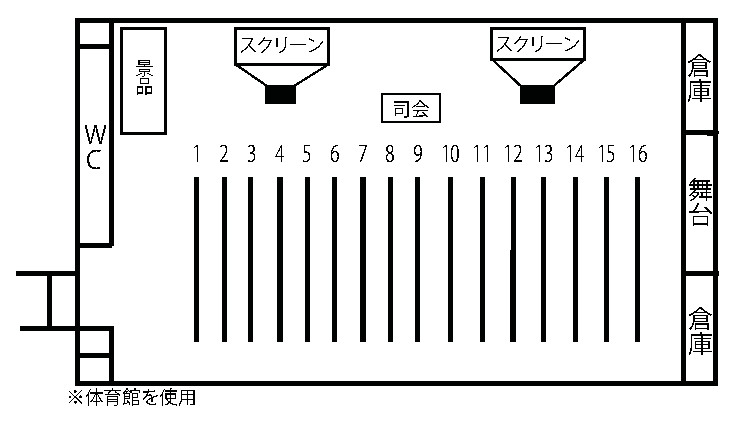
\includegraphics[width = 15cm]{./24/hyousyou.eps}
  \caption{退所式}
  \end{center}
\end{figure}

%%%%%%%%%%%%%%%%%%%%%%%%%%%%%%%%%%%%%%%%%%%%%%%%%%%%%%%%%%%%%%%%%%%%%%%%%%%%%%%
%\include{end}
